\documentclass[conference]{IEEEtran}
\IEEEoverridecommandlockouts

\usepackage{amsmath,amssymb,amsthm}
\usepackage{booktabs}
\usepackage{array}
\usepackage{cite}
\usepackage{url}
\usepackage{tikz}
\usetikzlibrary{arrows.meta,decorations.pathreplacing}
\usepackage[hidelinks]{hyperref}

\newtheorem{theorem}{Theorem}
\newtheorem{proposition}{Proposition}
\newtheorem{corollary}{Corollary}
\newtheorem{lemma}{Lemma}
\theoremstyle{definition}
\newtheorem{definition}{Definition}

\newcommand{\I}{I}
\newcommand{\Hh}{H}
\newcommand{\KL}{D_{\mathrm{KL}}}
\newcommand{\E}{\mathbb{E}}
\newcommand{\V}{\mathcal V}
\newcommand{\intuition}[1]{\noindent\textit{Intuition.} #1}

\begin{document}

\title{The Coffee Law: Information, Reasoning and\\Communication Ceilings for Tool-Using Agent Collectives}

\author{\IEEEauthorblockN{Manish Bhatt}
\IEEEauthorblockA{\emph{Affiliation to be completed}\\
\emph{email to be completed}}}

\maketitle

\begin{abstract}
Teams of LLM agents debate, vote and call tools in the hope of knowing more than
any one of them. We show that what such a team can achieve is limited by three
ceilings, each independent of how the agents work. \emph{Information}: a team
can never know more about the world than its starting data plus what its tools
can carry, $\min\{\Hh(\Theta),\,\I(\Theta;D_0)+\sum_t C_t\}$ bits, where $C_t$
is the capacity of round $t$'s tool calls; talking, voting and adding agents do
not raise this budget. \emph{Reasoning}: what computationally bounded agents can
\emph{use} is at most what they \emph{hold}; debate and extra compute close this
gap but never pass it, and closing it can cost anything from reading every input
to more than any efficient computation can supply. \emph{Communication}: when
data is split across agents, no single agent can use it without enough messages,
about $n/2$ bits for some $n$-bit tasks even with unlimited computation. The
ceilings explain a body of published findings: extra thinking fails on
knowledge-intensive tasks, debate helps on reasoning tasks but no more than
voting at equal compute, identical agents saturate, distributed information
goes unpooled, and models know only what their training carried. We also
formalize sandboxing as a guarantee on reachable channels. Every finite example
is verified exactly in public code.
\end{abstract}

\begin{IEEEkeywords}
multi-agent systems, LLM agents, tool use, information theory, channel
capacity, usable information, communication complexity
\end{IEEEkeywords}

\section{Introduction}

A team of LLM agents is paged about a production incident. Two questions arrive.
\emph{Which server is failing?} The answer is in live logs the team has not yet
read. \emph{Is this patch to the locking code correct?} The answer is fully
determined by code the team already has. A common belief is that adding agents,
rounds of debate or thinking time helps with both. It does not, and the reason
is precise: the two questions hit different ceilings.

The first is limited by \textbf{information}. No amount of discussion reveals
log lines nobody has fetched; only tool calls (reading logs, running queries)
do, and each call can carry only so much. The second is limited by
\textbf{reasoning}: the answer is already in hand, and the work is computing it.
A third limit appears when data is split across agents, since what one agent
holds is useless to another until it is communicated: \textbf{communication}.

This paper makes those three ceilings exact (Fig.~\ref{fig:ceilings}). The
mathematical tools are classical: the chain rule, the data-processing
inequality (DPI), channel capacity, Fano's inequality~\cite{cover2006}, usable
information~\cite{xu2020} and communication complexity~\cite{kushilevitz1997}.
What is new is their assembly into a theory of tool-using agent collectives,
which yields results not available from the textbook statements:
\begin{enumerate}
\item \textbf{A capacity budget for adaptive, multi-agent tool use} (the Coffee
Law, Theorem~\ref{thm:coffee}): the number of agents and the protocol drop out,
and Fano's inequality gives an error floor and a minimum number of tool calls,
including a worst-case version needing no prior.
\item \textbf{One chain for knowing and using}, usable $\le$ available $\le$
budget, with the gap between the first two equal to an expected KL divergence
(Theorem~\ref{thm:reasoning}), and bounds on the compute needed to close it
(Theorems~\ref{thm:compute}--\ref{thm:lower}).
\item \textbf{A communication ceiling for collectives}
(Theorem~\ref{thm:comm}), distinct from information and compute.
\item \textbf{A formal account of sandboxing}: reasoning can discover channels,
so a sandbox is a guarantee on which channels any feasible computation can reach
(Theorem~\ref{thm:gated}).
\item \textbf{A unified explanation of published findings}
(Table~\ref{tab:evidence}), and testable predictions.
\end{enumerate}
Full proofs and exact numerical checks of every finite example are
public.\footnote{\url{https://github.com/mbhatt1/coffeelaw}}

\begin{figure}[t]
\centering
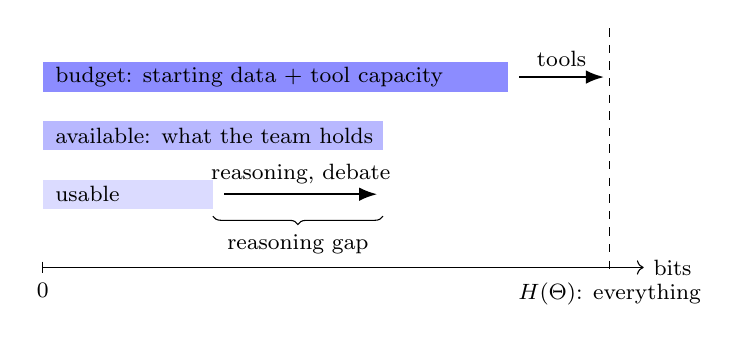
\begin{tikzpicture}[x=7.2cm,y=0.62cm,font=\footnotesize]
\draw[->] (0,0) -- (1.06,0) node[right] {bits};
\draw (0,0.12) -- (0,-0.12) node[below] {$0$};
\draw[dashed] (1,4.9) -- (1,-0.12) node[below] {$\Hh(\Theta)$: everything};
\fill[blue!45] (0,3.6) rectangle (0.82,4.2);
\fill[blue!28] (0,2.4) rectangle (0.60,3.0);
\fill[blue!14] (0,1.2) rectangle (0.30,1.8);
\node[anchor=west] at (0.005,3.9) {budget: starting data $+$ tool capacity};
\node[anchor=west] at (0.005,2.7) {available: what the team holds};
\node[anchor=west] at (0.005,1.5) {usable};
\draw[-{Latex},thick] (0.84,3.9) -- (0.99,3.9) node[midway,above] {tools};
\draw[-{Latex},thick] (0.32,1.5) -- (0.59,1.5)
  node[midway,above] {reasoning, debate};
\draw[decorate,decoration={brace,amplitude=3pt,mirror}]
  (0.30,1.05) -- (0.60,1.05) node[midway,below=3pt] {reasoning gap};
\end{tikzpicture}
\caption{The ceilings. What a team can use is at most what it holds, which is
at most its budget. Tools (and better starting data) raise the budget; reasoning
(more compute, debate, more agents) raises usable information toward what is
held, never past it. When data is split across agents, a third ceiling,
communication, limits what each agent can use.}
\label{fig:ceilings}
\end{figure}

The theory is agent-agnostic: it applies equally to people, programs and mixed
human--AI teams. It bounds learning about the world and using what is learned;
it does not cap intelligence, and it says nothing about outcomes the agents
themselves bring about.

\section{Model}\label{sec:model}

\intuition{We track one object: the \emph{record}, everything the team has
ever held. Each round, agents may call tools; tool answers depend on the world;
everything else the agents do (posting, debating, voting, thinking) is a
function of the record plus coin flips.}

\smallskip
All variables are discrete with finite support (Section~\ref{sec:ext} treats
continuous ones); logarithms are base~2. $\Theta$ is the truth the team wants.
$D_t$ is the record at the start of round $t$: the initial data $D_0$ (every
agent's context and model) plus every post, private state, query and tool result
since. In round $t$, internal randomness $\xi_t$ is drawn; tool calls
$Q_t=g_t(D_t,\xi_t)$ are issued under any policy; results
$O_{t+1}\sim K_t(\cdot\mid\Theta,Q_t,D_t)$ return; communication and computation
use fresh randomness $\zeta_t$; and $D_{t+1}=(D_t,\xi_t,Q_t,O_{t+1},\zeta_t)$.

\noindent\textbf{Assumptions.} (A1)~\emph{No side channels}: $\Theta$ reaches the
team only through $D_0$ and tool results. (A2)~\emph{Coin flips are honest}:
$\xi_t,\zeta_t$ are independent of $\Theta$ and of everything before them.
(A3)~\emph{Tools are channels from the world}: given $(\Theta,Q_t,D_t)$, $O_{t+1}$
has law $K_t$ (tools may be adaptive or stateful). (A4)~\emph{The truth is
fixed}: the team's actions do not change $\Theta$. Section~\ref{sec:ext}
relaxes each assumption.

\noindent\textbf{Capacity.} For each query $q$ and history $d$, the tool is a
channel $\theta\mapsto K_t(\cdot\mid\theta,q,d)$ with capacity
$\mathrm{Cap}(K_{t,q,d})=\max_{P}\I(\Theta;O)$, the most it can ever reveal per
call. Let $C_t=\sup_{q,d}\mathrm{Cap}(K_{t,q,d})$. Always
$C_t\le\min\{\log|\mathcal O_t|,\log|\mathrm{supp}\,\Theta|\}$; a pass/fail test
has $C_t\le 1$ bit.

\noindent\textbf{What is random.} For facts about the world, the randomness is
over \emph{possible worlds} $W$: a question $X\perp W$ has answer
$\Theta=\theta(W,X)$, and training is a channel $W\to\text{corpus}\to M$ to the
weights $M$. Then $\I(\Theta;X,M)\le\I(\Theta;X)+\I(W;M)$ and
$\I(W;M)\le\I(W;\text{corpus})$: a model knows at most what its training data
carried. In one fixed world, $M$ is constant and $\Theta$ is a function of $X$, so
a model's factual knowledge appears as \emph{usable} information
(Section~\ref{sec:reasoning}): something it computes from the question.

\section{Ceiling 1: Information (the Coffee Law)}\label{sec:coffee}

\intuition{Picture each tool call as a narrow pipe from the world into the
team's shared bucket. Talking, voting and thinking move water between cups; they
never add water. Only pipes do, and each pipe has a width.}

\begin{theorem}[Coffee Law]\label{thm:coffee}
Under (A1)--(A4), with $B_T=\I(\Theta;D_0)+\sum_{t<T}C_t$,
\[
\I(\Theta;D_T)\le\min\{\Hh(\Theta),B_T\},
\]
and the same holds for every output of the team (answer, vote, board, any
agent's state). For any estimator $\hat\Theta$ and $|\Theta|\ge3$,
$\Pr(\hat\Theta\ne\Theta)\ge(\Hh(\Theta)-\min\{\Hh(\Theta),B_T\}-1)/\log(|\Theta|-1)$.
In particular, with no tools, $\I(\Theta;D_T)\le\I(\Theta;D_0)$: a closed team
cannot learn anything by talking.
\end{theorem}

\begin{proof}
By the chain rule, a round adds
$\I(\Theta;\xi_t|D_t)+\I(\Theta;Q_t|D_t,\xi_t)+\I(\Theta;O_{t+1}|S)+\I(\Theta;\zeta_t|S,O_{t+1})$
with $S=(D_t,\xi_t,Q_t)$. The first and last terms are $0$ by (A2); the second
is $0$ because $Q_t$ is a function of $(D_t,\xi_t)$. Given $S=s=(d,x,q)$, (A3)
makes $(\Theta,O_{t+1})$ an input--output pair of channel $K_{t,q,d}$ with input
law $p(\cdot|s)$, so the third term is at most $\mathrm{Cap}(K_{t,q,d})\le C_t$.
Sum over rounds; also $\I\le\Hh$. Outputs are functions of $D_T$ and independent
noise (DPI). Fano's inequality gives the error floor.
\end{proof}

Choosing queries cleverly is already accounted for: a policy only selects which
channel to use and under which posterior, and capacity is the maximum over both,
as feedback cannot raise the capacity of a memoryless
channel~\cite{shannon1956,massey1990}.

\begin{corollary}[What does not help]\label{cor:agents}
Debate, voting, critique and the number of agents do not appear in $B_T$. More
agents raise the budget only by making more, or more informative, tool calls.
\end{corollary}

\begin{corollary}[Calls needed]\label{cor:rounds}
If $\Theta$ is uniform on $2^k$ values ($k\ge2$), $\I(\Theta;D_0)=0$ and $C_t\le
C$, then error $\le\varepsilon$ requires at least $((1-\varepsilon)k-1)/C$ tool
rounds, however many agents run and however they talk.
\end{corollary}

\noindent\textbf{Example: debugging.} A test run returns pass or fail, so it
carries at most one bit. Finding one bad commit among $n$ therefore needs about
$\log n$ test runs whatever the team does; binary search (\texttt{git bisect})
achieves this. A flaky test that misreports with probability $p$ carries at most
$1-h(p)$ bits, raising the minimum by the factor $1/(1-h(p))$.

\noindent\textbf{Exact accounting and tightness.} The proof gives the identity
$\I(\Theta;D_T)=\I(\Theta;D_0)+\sum_t\E_s[\I(\Theta;O_{t+1}|S_t=s)]$: total
information is the sum of what each call actually revealed. The bound is tight
exactly when every call is used at full capacity, i.e.\ almost every posterior
is a capacity-achieving input for the chosen tool. For rich tools (a web page),
the realized per-call gain is the binding quantity; the capacity form bites for
low-capacity tools such as tests, checks and short API answers.
Table~\ref{tab:tight} shows a case where a good policy meets the bound and a
poor one wastes it.

\begin{table}[t]
\caption{Exact information after two tool rounds. $\Theta$ is uniform on 4
values; each call returns one chosen bit of $\Theta$, flipped with probability
$0.1$ ($C\approx0.531$ bits).}
\label{tab:tight}
\centering
\begin{tabular}{@{}lcc@{}}
\toprule
Policy & $\I(\Theta;D_2)$ & Budget \\
\midrule
Ask bit 0, then bit 1 & 1.0620 & 1.0620 \\
Adaptive, may repeat a bit & 0.9820 & 1.0620 \\
Either, plus a debate step & unchanged & --- \\
Ask both bits, noise-free tool & 2.0000 & 2.0000 \\
\bottomrule
\end{tabular}
\end{table}

\section{Ceiling 2: Reasoning}\label{sec:reasoning}

\intuition{Holding information is not the same as using it. The prime factors
of a number $N$ are completely determined by $N$, so a team holding $N$ holds
all the information about them; finding them may still take enormous
computation. Reasoning turns held information into usable information.}

\begin{definition}[\cite{xu2020}]
A \emph{predictive family} $\V$ is a set of predictors $f$ mapping a record $d$
to a distribution $f[d]$ on $\Theta$, including the prior predictor; it models
what the agents can compute. Let
$\Hh_\V(\Theta|D)=\inf_{f\in\V}\E[-\log f[D](\Theta)]$ and define the
\emph{usable information} $\I_\V(D\to\Theta)=\Hh(\Theta)-\Hh_\V(\Theta|D)$.
\end{definition}

\begin{theorem}[Reasoning ceiling]\label{thm:reasoning}
(a)~$0\le\I_\V(D\to\Theta)\le\I(\Theta;D)$, with \emph{reasoning gap}
$\I(\Theta;D)-\I_\V(D\to\Theta)=\inf_{f\in\V}\E_D\,\KL(p(\cdot|D)\,\|\,f[D])$.
(b)~Hence $\I_\V(D_T\to\Theta)\le\I(\Theta;D_T)\le\min\{\Hh(\Theta),B_T\}$.
(c)~Computation can raise usable information but never available information:
for some $\V$ and deterministic $g$, $\I(\Theta;g(D))=\I(\Theta;D)$ while
$\I_\V(g(D)\to\Theta)>\I_\V(D\to\Theta)$; for every $g$,
$\I_\V(g(D)\to\Theta)\le\I(\Theta;D)$.
\end{theorem}

\begin{proof}
(a)~The prior predictor gives $\Hh_\V\le\Hh(\Theta)$. For any $f$,
$\E[-\log f[D](\Theta)]=\Hh(\Theta|D)+\E_D\KL(p(\cdot|D)\|f[D])$; take the
infimum. (b)~Part~(a) and Theorem~\ref{thm:coffee}. (c)~Let two agents hold
uniform bits $B_1,B_2$ and $\Theta=B_1\oplus B_2$, and let $\V$ read one
coordinate of the record. Each bit alone is independent of $\Theta$, so usable
information is $0$, although the pair determines $\Theta$. After one reasoning
step $g(D)=(B_1\oplus B_2,B_2)$, one coordinate equals $\Theta$: usable
information is $1$ bit, available information unchanged. The last claim is (a)
and the DPI.
\end{proof}

\begin{corollary}[Debate adds reasoning, not facts]\label{cor:debate}
In a closed team every post is a function of $D_0$ and noise, so it adds no
available information; it can add usable information, as when an agent posts an
intermediate result (here $B_1\oplus B_2$) that others could not compute. The
gain is capped by what the team holds.
\end{corollary}

The incident example is now exact. ``Which server is failing?'' is
\emph{information-bound}: the right inequality of the chain binds, and only
tools help. ``Is this patch correct?'' is \emph{compute-bound}: the left gap is
large, and reasoning helps. A code interpreter run on data already held is
reasoning (it enlarges $\V$); a tool that observes the world is information (it
raises $C_t$). In Table~\ref{tab:tight}'s noisy example, the record holds 1.062
bits but a one-look agent can use only 0.266; the rest is a reasoning gap that
more observations cannot close.

\noindent\textbf{Imperfect agents.} Real agents fall further below the chain
(proofs in the accompanying notes, footnote~1). Acting on a belief $\hat b$ instead of the
correct posterior $b^*$ costs at most $2U\,\mathrm{TV}(b^*,\hat b)+\delta\le
2U\sqrt{(\ln2/2)\KL(b^*\|\hat b)}+\delta$ for utility range $U$ and own
suboptimality $\delta$. A summary $M$ of data $D$ loses exactly
$\E\,\KL(p(\cdot|D)\|p(\cdot|M))=\I(\Theta;D)-\I(\Theta;M)$. And a confident
message carrying zero information can flip a correct agent: with belief
$(0.6,0.4)$ for the truth, giving weight $\alpha>1/6$ to a constant false claim
flips the answer.

\section{Paying for Reasoning}\label{sec:compute}

\intuition{Closing the reasoning gap costs computation. A team of agents is just
a computation spread over several machines, so what counts is total work; and
some tasks need a lot of it.}

\smallskip
Let $\V_S$ be the predictors computable and samplable in at most $S$ steps of a
fixed machine model (reading one input symbol per step). A team's \emph{total
compute} is the sum of all agents' steps over all rounds, counting board reads
and writes.

\begin{theorem}[Only total compute counts]\label{thm:compute}
A team with total compute $S$ outputs a predictor in $\V_{\kappa S}$ for a
constant $\kappa$ of the machine model, so its usable information is at most
$\I_{\V_{\kappa S}}(D\to\Theta)\le\I(\Theta;D)$.
\end{theorem}
\begin{proof}
One machine can run the agents step by step, keeping their memories and the
board in separate regions, at $O(1)$ cost per simulated step.
\end{proof}

\begin{lemma}\label{lem:guess}
Sampling $\hat\Theta\sim f[D]$ is correct with probability at least
$2^{-\E[-\log f[D](\Theta)]}$ (Jensen). If $\Hh(\Theta)\le1$, usable information
$\delta$ gives success probability at least $\frac12+\frac{\ln2}{2}\delta$.
\end{lemma}

\begin{theorem}[Some gaps are expensive]\label{thm:lower}
(a)~For the parity $\Theta$ of $n$ uniform bits, any predictor or team that
reads at most $n-1$ bits, even adaptively, has zero usable information; reading
all $n$ gives one bit. (b)~If one-way permutations exist, then for the
Goldreich--Levin bit $\Theta=\langle x,r\rangle\bmod 2$ given $D=(f(x),r)$,
$\I(\Theta;D)=\Hh(\Theta)$, yet every polynomial-time team has usable information
at most $\log(1+2\varepsilon(n))$ with $\varepsilon$ negligible.
\end{theorem}
\begin{proof}
(a)~Given any transcript of fewer than $n$ reads, the unread bits are uniform,
so $\Theta$ is independent of the transcript; posts are functions of their
authors' reads. (b)~Every polynomial-time algorithm guesses $\Theta$ with
probability at most $\frac12+\varepsilon$~\cite{goldreich1989}; apply
Lemma~\ref{lem:guess}; by Theorem~\ref{thm:compute} this covers any
polynomial-time team.
\end{proof}

\noindent So splitting work across agents buys speed, not capability, and
reaching the reasoning ceiling can cost anything from reading the whole input to
more than any efficient team can supply. No general formula exists in between
without resolving open problems such as P vs NP.

\section{Ceiling 3: Communication}\label{sec:comm}

\intuition{Two agents each hold half a puzzle. The team as a whole holds the
answer, but neither agent can use it until enough of the other half arrives.
For some puzzles a one-bit summary suffices; for others, nothing much shorter
than the data itself will do.}

\begin{theorem}[Communication ceiling]\label{thm:comm}
(a)~If the messages reaching agent~1 take at most $2^L$ values, then
$\I(\Theta;D^1,\Pi)\le\I(\Theta;D^1)+L$. (b)~If agents 1 and 2 hold uniform
$x,y\in\{0,1\}^n$ and $\Theta=\langle x,y\rangle\bmod2$, then
$\I(\Theta;x,y)=\Hh(\Theta)$, yet any protocol exchanging $L$ bits gives
$\I(\Theta;x,\Pi)\le\log(1+2^{L+1-n/2})$, even with unlimited computation.
\end{theorem}
\begin{proof}
(a)~$\I(\Theta;\Pi|D^1)\le\Hh(\Pi)\le L$. (b)~Append agent~1's output as one more
bit. Inner product has discrepancy at most $2^{-n/2}$ (Lindsey's
lemma~\cite{chor1988,kushilevitz1997}), so an $(L{+}1)$-bit protocol is correct
with probability at most $\frac12+2^{L-n/2}$; apply Lemma~\ref{lem:guess} to
agent~1's exact posterior.
\end{proof}

\noindent Parity splits cheaply (each agent posts one bit); inner product needs
about $n/2$ bits. This ceiling holds even when information and compute are
unlimited.

\section{Beyond the Assumptions}\label{sec:ext}

Each result relaxes one assumption; full proofs and exact checks are in the
accompanying notes (footnote~1).

\begin{theorem}[Reasoning can open channels: sandboxes]\label{thm:gated}
Let $A_S(d)$ be the queries a team can issue from record $d$ within compute $S$.
Then $\I(\Theta;D_T)\le\I(\Theta;D_0)+\sum_t\sup_{d,\,q\in A_S(d)}\mathrm{Cap}(K_{t,q,d})$,
nondecreasing in $S$. If a tool reveals a uniform 2-bit $\Theta$ only after a
uniform $k$-bit password is found, $S$ guesses give exactly
$\min\{1,S/2^k\}\cdot2$ bits.
\end{theorem}
\noindent So ``reasoning never adds information'' holds for a \emph{fixed} set of
reachable channels. Discovering an endpoint, credential or exploit is
computation that raises the budget. A \emph{sandbox} is a guarantee that every
feasible computation stays within allowed channels; an escape violates it. In
recently reported incidents, models under evaluation left their test sandbox
and retrieved benchmark answers from an outside server~\cite{openai2026}: the
answers were not inside, so the only route was an unallowed channel.

\noindent\textbf{Worst case.} For $M\ge3$ possible truths with no prior, starting
data of capacity $C_0$, and any strategy, some truth $\theta_i$ has
$\Pr_{\theta_i}(\hat\Theta\ne\theta_i)\ge(\log M-\min\{\log M,C_0+\sum_tC_t\}-1)/\log(M-1)$
(Fano's method). The law holds for specific tasks, not only on average.

\noindent\textbf{Acting.} In a fixed unknown environment $W$ with $M\ge3$
actions, a unique best action $A^*$ and gap $\Delta$, round-$t$ regret is at least
$\Delta(\Hh(A^*)-\min\{\Hh(A^*),\I(W;D_0)+\sum_{s<t}C_s\}-1)/\log(M-1)$: the
action is an estimate of $A^*$. Taking $W$ to be a user's hidden specification
covers open-ended work: an agent cannot reliably build what it has not learned
the user wants.

\noindent\textbf{A changing world.} If $\Theta_t$ drifts as a Markov chain with
strong data-processing constant $\eta<1$~\cite{ahlswede1976}, and tools observe
the current state, then $\I(\Theta_t;D_t)\le\eta^t\I(\Theta_0;D_0)+\eta C/(1-\eta)$:
knowledge saturates however long agents run.

\noindent\textbf{Adversaries and provenance.} If every post is stored with its
author, adversarial posts cannot reduce available information:
$\I(\Theta;D,M)\ge\I(\Theta;D)$. Without attribution one adversary can erase it:
if an honest agent posts a fair bit $\Theta$ and an adversary posts $1-\Theta$,
the unattributed record carries 0 bits. Authenticate and attribute messages.

\noindent\textbf{Continuous truths.} For real $\Theta$ the budget holds with
capacities under input constraints, and every estimator has
$\E[(\Theta-\hat\Theta)^2]\ge(2\pi e)^{-1}2^{2(h(\Theta)-B_T)}$, with equality for
a Gaussian truth in Gaussian noise: each bit divides the best squared error by 4.

\noindent\textbf{Where to spend.} From the chain: extra reasoning on the same
record can raise usable information by at most the reasoning gap
$\I(\Theta;D)-\I_\V(D\to\Theta)$, and extra tool rounds can raise available
information by at most $\sum C_t$. A spending rule follows: invest in the lever
whose headroom per unit cost is larger, and stop investing in a lever whose
headroom is exhausted.

\noindent\textbf{Measuring the quantities.} Usable information is estimable:
$\Hh(\Theta)$ minus the held-out log-loss of a team's calibrated predictions
lower-bounds $\I_\V$, with PAC guarantees under computational
constraints~\cite{xu2020}. Tool capacity is bounded by the answer space, and for
noisy tools by measured error rates (a test that flakes with probability $p$ has
$C\le1-h(p)$). Available information about the world, $\I(W;M)$ for a pretrained
model, is well defined but hard to estimate; the bounds' value is then
structural rather than numerical.

\section{Evidence and Predictions}\label{sec:empirical}

Table~\ref{tab:evidence} lists predictions of the theory and published findings
that bear on them. None contradicts it. Two points deserve care. First, the
theory does not predict that debate is worse than other methods; it predicts
that debate is worth its compute, so at matched compute it should perform about
as well as self-consistency or voting. Small gaps in either
direction~\cite{tran2026,smit2024,choi2025} are consistent with this. Second,
some findings look like tensions. Debate is reported to improve
\emph{factuality}~\cite{du2024}; but within the actual world a factual answer is
determined by the question, so this is reasoning over stored knowledge, not new
information. Debate is proved not to help Bayesian agents~\cite{choi2025}; such
agents have no reasoning gap, so Theorem~\ref{thm:reasoning} predicts exactly
that.

\begin{table*}[t]
\caption{Predictions of the theory and published evidence. Findings are from
the cited papers' abstracts and published summaries.}
\label{tab:evidence}
\centering
\footnotesize
\begin{tabular}{@{}p{4.4cm}p{9.6cm}p{2.0cm}@{}}
\toprule
Prediction (result in this paper) & Published finding & Verdict \\
\midrule
Extra thinking does not help information-bound tasks (Thm.~\ref{thm:coffee}, no tools)
 & More test-time compute does not reliably raise closed-book accuracy across 14 reasoning models and often increases hallucination~\cite{zhao2026}; self-correction without external feedback often fails~\cite{huang2024}. & Supported \\
Tools raise information-bound accuracy (Thm.~\ref{thm:coffee})
 & Retrieval and tool use are the standard remedy for knowledge-intensive tasks~\cite{lewis2020,yao2023,schick2023}. & Supported \\
A model knows only what its training carried (Sec.~\ref{sec:model})
 & QA accuracy tracks the number of relevant pretraining documents, causally; retrieval reduces the dependence~\cite{kandpal2023}. & Supported \\
Debate helps compute-bound tasks (Thm.~\ref{thm:reasoning})
 & Debate improves mathematical and strategic reasoning~\cite{du2024}. & Supported \\
Debate is worth its compute, no more (Cor.~\ref{cor:debate})
 & Debate does not reliably beat self-consistency~\cite{smit2024}; most gains come from voting~\cite{choi2025}; single agents match multi-agent systems at equal thinking tokens~\cite{tran2026}. & Consistent \\
More identical agents saturate (Thm.~\ref{thm:compute}, Cor.~\ref{cor:agents})
 & Homogeneous agents show strong diminishing returns; two diverse agents can match sixteen identical ones~\cite{yang2026}; voting gains grow with task difficulty~\cite{li2024agents}. & Supported \\
Redundant tool calls add little (Thm.~\ref{thm:coffee}, exact accounting)
 & Accuracy plateaus after about eight calls and redundant calls can hurt~\cite{du2025infomosaic}. & Supported \\
Split information must be communicated (Thm.~\ref{thm:comm})
 & Agent groups reach 30.1\% with distributed information versus 80.7\% for one agent with all of it; agents do not seek what others hold~\cite{li2026hidden}. & Supported \\
Zero-information messages flip correct agents (Sec.~\ref{sec:reasoning})
 & Debate can lower accuracy over time as agents switch from correct to incorrect answers~\cite{wynn2025}. & Supported \\
Without provenance, adversaries erase information (Sec.~\ref{sec:ext})
 & Stealthy tampering of inter-agent messages succeeds across tasks and architectures~\cite{yan2026mast}. & Supported \\
In a changing world knowledge decays and tools refresh it only partly (Sec.~\ref{sec:ext})
 & Under continuous knowledge drift, retrieval and learning methods struggle~\cite{liu2026drift}. & Supported \\
Open-ended work is bounded by information about intent (Sec.~\ref{sec:ext})
 & Underspecification consistently hurts agents; an ask-user tool recovers part of the loss~\cite{pu2026lhaw}. & Supported \\
Error vs.\ informative tool calls stays above the Fano floor (Cor.~\ref{cor:rounds})
 & Not yet measured. & Open \\
\bottomrule
\end{tabular}
\end{table*}

\noindent\textbf{Testable predictions.} (P1)~Error rate against the number of
informative tool calls stays above the floor of Corollary~\ref{cor:rounds}; a
clean test uses a yes/no tool with known noise, where the floor is exact.
(P2)~At matched compute, debate performs about as well as self-consistency or
voting; it helps compute-bound tasks and not information-bound ones, while tools
show the opposite pattern. (P3)~Redundant or low-capacity tool calls add
little, however numerous. (P4)~With data split across agents, accuracy on tasks
like inner product stays near chance until the message budget approaches the
communication ceiling of Theorem~\ref{thm:comm}.

\section{Related Work}

Closed-system debate is bounded via the DPI in~\cite{shin2026} and modeled as a
belief martingale in~\cite{choi2025}. Yang~et~al.~\cite{yang2026} bound
multi-agent performance by task uncertainty and a sum of per-agent channel
informations, the same ``$\min\{\Hh,\sum\text{channels}\}$'' shape with agents as
the channels. Fano-type bounds have been applied to queries in adversarial
attacks~\cite{kaneko2025} and to single-pass multi-hop reasoning~\cite{wan2026fano}.
Usable information is due to~\cite{xu2020}; synergy is studied in partial
information decomposition~\cite{williams2010}; feedback and directed information
in~\cite{massey1990}; and Fano-based active-learning bounds
in~\cite{raginsky2011}. To our knowledge, the per-call capacity budget for
adaptive multi-agent tool use, its combination with usable information and
communication into one set of ceilings, and the channel account of sandboxing
have not been stated before.

\section{Limitations}

The bounds concern information about a world the agents do not change; outcomes
the team itself brings about need a different theory. The ceilings hold
separately, but how to trade one for another is open, as is modeling agents'
incentives (reward hacking, goal adoption), which the bounds do not address.
Bounds for agents that learn across episodes, whose starting data changes over
time, are not given. Equality in Theorem~\ref{thm:coffee} is characterized, but no
general algorithm achieves it. The proofs are mathematical and checked
numerically on finite examples, not machine-verified. We report no new
experiments; Table~\ref{tab:evidence} relies on published findings, summarized
from their abstracts.

\section{Conclusion}

A team of agents can be clever, but it cannot know more than it has seen, use
more than it holds, or combine what its members hold without communicating
enough. For practitioners the theory reduces to one question per task:
\emph{which ceiling binds?} If the answer is not in the data, add better
observations of the world. If it is in the data, add reasoning, and expect
debate to be worth exactly the compute it spends. If it is split across agents,
make sure they can say enough to each other. And treat sandboxes and message
provenance as channel control, because channels are where information comes
from.

\bibliographystyle{IEEEtran}
\bibliography{refs}

\end{document}
